%%%%%%%%%%%%%%%%%%%%%%%%%%%%%%%%%%%%%%%%%
% Academic Title Page
% LaTeX Template
% Version 2.0 (17/7/17)
%
% This template was downloaded from:
% http://www.LaTeXTemplates.com
%
% Original author:
% WikiBooks (LaTeX - Title Creation) with modifications by:
% Vel (vel@latextemplates.com)
%
% License:
% CC BY-NC-SA 3.0 (http://creativecommons.org/licenses/by-nc-sa/3.0/)
%
%%%%%%%%%%%%%%%%%%%%%%%%%%%%%%%%%%%%%%%%%

%----------------------------------------------------------------------------------------
%	PACKAGES AND OTHER DOCUMENT CONFIGURATIONS
%----------------------------------------------------------------------------------------

\documentclass[11pt]{article}

\usepackage[utf8]{inputenc} % Required for inputting international characters
\usepackage[T1]{fontenc} % Output font encoding for international characters
\usepackage{mathpazo} % Palatino font
\usepackage{amsmath}
\usepackage{tikz}
\usepackage{mathdots}
\usepackage{yhmath}
\usepackage{cancel}
\usepackage{color}
\usepackage{siunitx}
\usepackage{array}
\usepackage{multirow}
\usepackage{amssymb}
\usepackage{gensymb}
\usepackage{tabularx}
\usepackage{booktabs}
\usetikzlibrary{fadings}
\usetikzlibrary{patterns}
\usetikzlibrary{shadows.blur}

\begin{document}

%----------------------------------------------------------------------------------------
%	TITLE PAGE
%----------------------------------------------------------------------------------------

\begin{titlepage} % Suppresses displaying the page number on the title page and the subsequent page counts as page 1
	\newcommand{\HRule}{\rule{\linewidth}{0.5mm}} % Defines a new command for horizontal lines, change thickness here
	
	\center % Centre everything on the page
	
	%------------------------------------------------
	%	Headings
	%------------------------------------------------
	
	\textsc{\LARGE Polytech Nice Sophia}\\[1.5cm] % Main heading such as the name of your university/college
	
	\textsc{\Large Projet SI4 - Algorithmes et Complexité.}\\[0.5cm] % Major heading such as course name
	
	\textsc{\large Rapport de projet}\\[0.5cm] % Minor heading such as course title
	
	%------------------------------------------------
	%	Title
	%------------------------------------------------
	
	\HRule\\[0.4cm]
	
	{\huge\bfseries Algorithmes pour l'inférence de connectivité avec application en biologie structurale computationnelle}\\[0.4cm] % Title of your document
	
	\HRule\\[0.6cm]

		
	%------------------------------------------------
	%	Logo
	%------------------------------------------------
	
	\vfill
	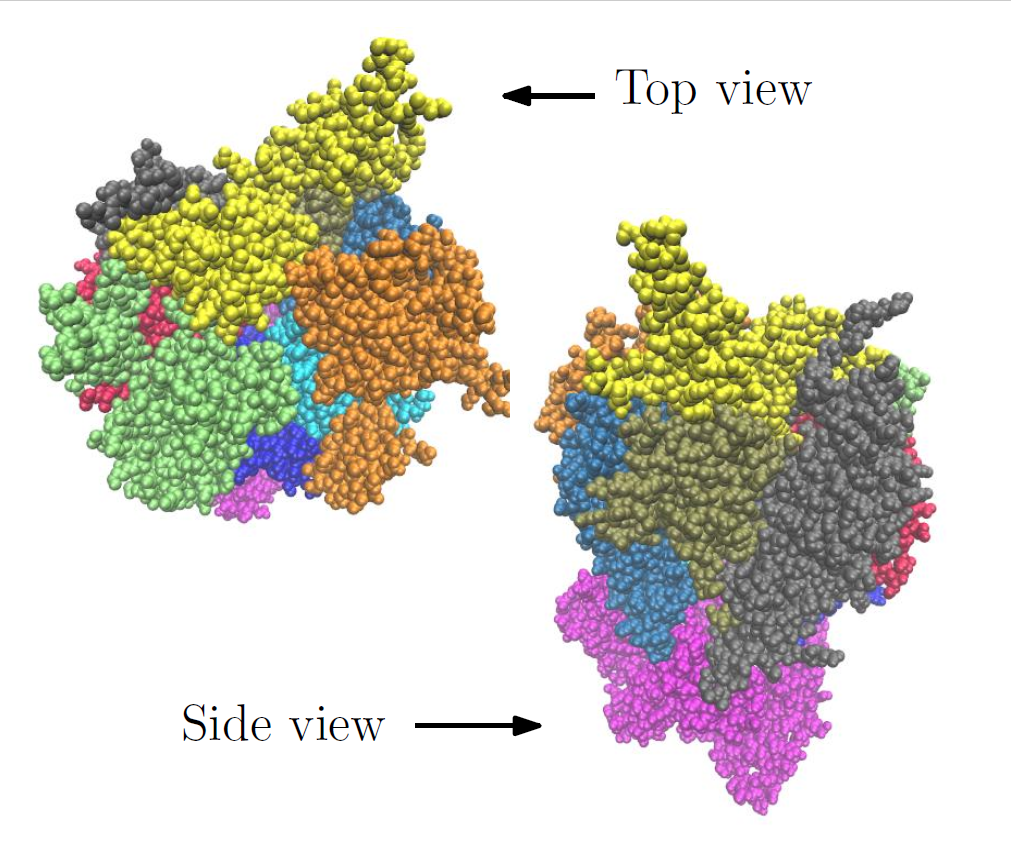
\includegraphics[width=0.6\textwidth]{complex.png}\\[1cm] % Include a department/university logo - this will require the graphicx package
	
	%------------------------------------------------
	%	Author(s)
	%------------------------------------------------
	
	\begin{minipage}{0.4\textwidth}
		\begin{flushleft}
			\large
			\textit{Author}\\
			Louis \textsc{Amas} % Your name 

			Maxime \textsc{Leras} % Your name
		\end{flushleft}
	\end{minipage}
	~
	\begin{minipage}{0.4\textwidth}
		\begin{flushright}
			\large
			\textit{Author}\\
			Pierre-Antoine \textsc{Boulat} % Supervisor's name
			Julien \textsc{Molinier} % Supervisor's name
		\end{flushright}
	\end{minipage}
	
	
	% If you don't want a supervisor, uncomment the two lines below and comment the code above
	%{\large\textit{Author}}\\
	%John \textsc{Smith} % Your name
	
	%------------------------------------------------
	%	Date
	%------------------------------------------------
	
	\vfill\vfill\vfill\vfill % Position the date 3/4 down the remaining page
	
	{\large\today} % Date, change the \today to a set date if you want to be precise

	 
	%----------------------------------------------------------------------------------------
	
	\vfill % Push the date up 1/4 of the remaining page
	
\end{titlepage}

%----------------------------------------------------------------------------------------

\newpage

\section{Question 1}
\paragraph{}
\begin{equation}
	Pour \; \Delta = 3 : 
\end{equation}

Une solution existe avec :

\begin{equation}
	\Delta(G) = deg({\widehat{S}_2}) = deg({\widehat{S}_4}) = 3
\end{equation}

\paragraph{}
\tikzset{every picture/.style={line width=0.75pt}} %set default line width to 0.75pt        

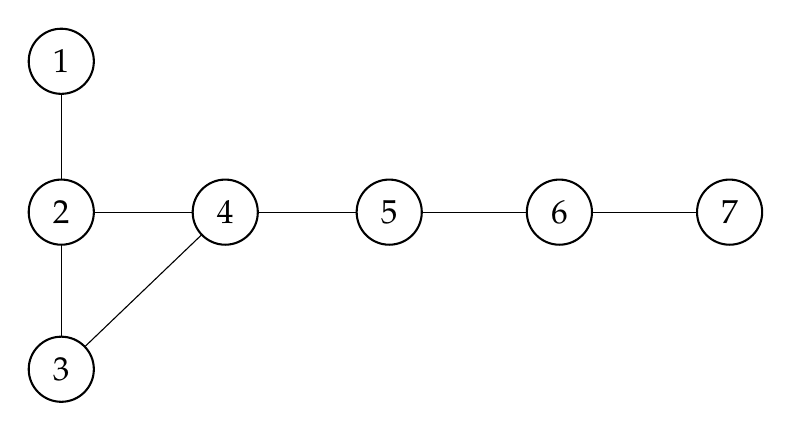
\begin{tikzpicture}[x=0.75pt,y=0.75pt,yscale=-1,xscale=1]
%uncomment if require: \path (0,232.6750030517578); %set diagram left start at 0, and has height of 232.6750030517578

% Text Node
\draw  [line width=0.75]   (168, 41.31) circle [x radius= 15.69, y radius= 15.69]   ;
\draw (168,41.31) node  [font=\large] [align=left] {1};
% Text Node
\draw  [line width=0.75]   (168, 189.69) circle [x radius= 15.69, y radius= 15.69]   ;
\draw (168,189.69) node  [font=\large] [align=left] {3};
% Text Node
\draw  [line width=0.75]   (168, 114) circle [x radius= 15.69, y radius= 15.69]   ;
\draw (168,114) node  [font=\large] [align=left] {2};
% Text Node
\draw  [line width=0.75]   (247, 114) circle [x radius= 15.69, y radius= 15.69]   ;
\draw (247,114) node  [font=\large] [align=left] {4};
% Text Node
\draw  [line width=0.75]   (326, 114) circle [x radius= 15.69, y radius= 15.69]   ;
\draw (326,114) node  [font=\large] [align=left] {5};
% Text Node
\draw  [line width=0.75]   (408, 114) circle [x radius= 15.69, y radius= 15.69]   ;
\draw (408,114) node  [font=\large] [align=left] {6};
% Text Node
\draw  [line width=0.75]   (490, 114) circle [x radius= 15.69, y radius= 15.69]   ;
\draw (490,114) node  [font=\large] [align=left] {7};

% Connection
\draw    (168,57) -- (168,98.31) ;
% Connection
\draw    (168,129.69) -- (168,174) ;
% Connection
\draw    (183.69,114) -- (231.31,114) ;
% Connection
\draw    (262.69,114) -- (310.31,114) ;
% Connection
\draw    (341.69,114) -- (392.31,114) ;
% Connection
\draw    (423.69,114) -- (474.31,114) ;
% Connection
\draw    (179.33,178.84) -- (235.67,124.86) ;

\end{tikzpicture}


\paragraph{}
\begin{equation}
	Pour \; \Delta = 2 : 
\end{equation}

	Pas de solution car les sommets 4 et 5 sont présent dans 3 sous complexes, 
	ce qui force un degrée minimal sur ces sommets de 3

\begin{equation}
	\left | C_b \cap C_c \cap C_d \right | = 2 \;\; < 3
\end{equation}

\section{Question 2}
\paragraph{}
Lorsque $\Delta = | V |$, il existe une solution au problème IC lorsque

\begin{equation}
	k \geq (\sum_{i=1}^{t} | C_i |) - t
\end{equation}

Ces valeurs de $k$ ne sont vraies qu'en faisant la supposition que 

$|C_i \cap C_j| \leq 1$ pour tout $i \in \left\{1,...,t\right\}$ et pour tout
 $j \in \left\{1,...,t\right\} , i\ne j.$

 \paragraph{}
 En effet, si on avait $|C_i \cap C_j| > 1$, la valeur de $k$ minimale pour que 
le problème IC ait une solution serait inférieure à la valeur donnée en (5)
	

\newpage
\paragraph{}
Si $k = |V|^2$, on observe qu'un graphe complet a au plus $\frac{n*(n+1)}{2}$ arrêtes où $n = |V|$

Or $\forall n \geq 1, \frac{n*(n+1)}{2} \leq n^2$ , Cela revient donc à ne pas se préoccuper de $k$ 
car $|E|$ ne pourra jamais être supérieur à $k$

Les valeurs de $\Delta$ pour lesquelles IC a une solution sont donc toutes les valeurs
supérieures ou égales au nombre maximal d'occurences d'un sommet dans tous les sous-complexes

\paragraph{}
Si on prend l'exemple d'un assemblage dont tous les sous-complexes contiennent le même sommet $\widehat{S}_1$,
toujours en respectant la supposition de l'énoncé : $|C_i \cap C_j| \leq 1$ pour tout $i \in \left\{1,...,t\right\}$ et pour tout
$j \in \left\{1,...,t\right\} , i\ne j.$

On obtient un graphe en forme "d'étoile" avec pour centre le sommet $\widehat{S}_1$. Pour que IC ait une solution
dans cette instance, il faut $\Delta = t$ car $t$ est le nombre maximal d'occurences d'un sommet dans les sous-ensembles
et ce sommet est ici $\widehat{S}_1$

\section{Question 3}
\paragraph{}
Le nombre d'abres couvrants différents pour un graphe complet $G(V,E)$ à $p$ sommets peut directement être calculé
avec la formule de Cayley et on obtient :

\begin{equation}
	a(G) = p^{p-2} 
\end{equation}




\end{document}
